% This must be in the first 5 lines to tell arXiv to use pdfLaTeX, which is strongly recommended.
\pdfoutput=1
% In particular, the hyperref package requires pdfLaTeX in order to break URLs across lines.

\documentclass[11pt]{article}

% Remove the "review" option to generate the final version.
\usepackage[]{emnlp2021}

% Standard package includes
\usepackage{times}
\usepackage{latexsym}

% For proper rendering and hyphenation of words containing Latin characters (including in bib files)
\usepackage[T1]{fontenc}
% For Vietnamese characters
% \usepackage[T5]{fontenc}
% See https://www.latex-project.org/help/documentation/encguide.pdf for other character sets

% This assumes your files are encoded as UTF8
\usepackage[utf8]{inputenc}

% This is not strictly necessary, and may be commented out,
% but it will improve the layout of the manuscript,
% and will typically save some space.
\usepackage{microtype}

% If the title and author information does not fit in the area allocated, uncomment the following
%
%\setlength\titlebox{<dim>}
%
% and set <dim> to something 5cm or larger.

%%%%%%%%%%%%%%%%%%%%%%%%%%%%%%%%%%%%%%%%%%%%%%%%%%
% CUSTOM PACKAGES
%%%%%%%%%%%%%%%%%%%%%%%%%%%%%%%%%%%%%%%%%%%%%%%%%%

\usepackage{amsfonts}

%%%%%%%%%%%%%%%%%%%%%%%%%%%%%%%%%%%%%%%%%%%%%%%%%%
% TABLES, FIGURES, CHARTS...
%%%%%%%%%%%%%%%%%%%%%%%%%%%%%%%%%%%%%%%%%%%%%%%%%%

%\usepackage{subcaption}
\usepackage{graphicx}
\usepackage{tikz}
\usepackage{tikz-dependency}
\usetikzlibrary{shapes.geometric,calc}
\usetikzlibrary{colorbrewer}
\usepackage{caption}
\usepackage{subcaption}
% Multirows in tables
\usepackage{multirow}
\usepackage{tabularx}
\usepackage{booktabs}
\usepackage[normalem]{ulem}
\useunder{\uline}{\ul}{}
\usepackage{float}
\usepackage{pgfplots}
\pgfplotsset{compat=1.14, every non boxed x axis/.append style={x axis line style=-},
     every non boxed y axis/.append style={y axis line style=-}}


%%%%%%%%%%%%%%%%%%%%%%%%%%%%%%%%%%%%%%%%%%%%%%%%%%
% MACROS
%%%%%%%%%%%%%%%%%%%%%%%%%%%%%%%%%%%%%%%%%%%%%%%%%%
\newcommand{\todo}[1]{{\color{red}\textbf{[[TODO: #1]]}}}

\newcommand{\BigO}[1]{\ensuremath{\operatorname{O}\bigl(#1\bigr)}}

%%%%%%%%%%%%%%%%%%%%%%%%%%%%%%%%%%%%%%%%%%%%%%%%%%
% OTHERS
%%%%%%%%%%%%%%%%%%%%%%%%%%%%%%%%%%%%%%%%%%%%%%%%%%
\usepackage{lipsum}     % lorem ipsum
\urlstyle{same}           % pretty urls...
%\hypersetup{urlcolor=black}
\usepackage{enumitem}% http://ctan.org/pkg/enumitem
\usepackage{mathtools}


%%%%%%%%%%%%%%%%%%%%%%%%%%%%%%%%%%%%%%%%%%%%%%%%%%
% TITLE SETUP
%%%%%%%%%%%%%%%%%%%%%%%%%%%%%%%%%%%%%%%%%%%%%%%%%%

\title{
	ZPJa: Reinvent the Wheel - GRU\\
	\large{Project report}
}

\author{Svätopluk Hanzel \\
  \texttt{xhanze10@stud.fit.vut.cz} \\\And
  Martin Dočekal\\
  \texttt{idocekal@fit.vutbr.cz}
 }

\begin{document}
	\maketitle
	\begin{abstract}
		In this project I succesfully implemented a simple GRU neural network for character prediction from scratch including forward and backward passes, and advanced optimizer.
		
		It was then tested on several datasets with different size and complexity as well as various optimizers and different hyperparameter settings. All of these results are presented in this report.
	\end{abstract}


	\section{Task Definition}
		The task in this specific variant of the assignment was to implement a GRU RNN without using any preexisting library or tools and implementing both forward and backward passes.
		
		This network is then to be used and tested on a simple dataset for demonstrational purposes.
	
	\section{Introduction} \label{sec:introduction}
		The main goal of this project is to get hands-on experience with GRU RNN networks on a low level, thus increasing my understanding of them. This is reflected in the tools, programming language, and the overall approach to this project.
		
		Recurrent neural networks (RNN) are a class of artificial neural networks adapted to work with for time series -- by connecting neurons in loops they allow the network to keep the information of previous inputs for the latter ones.
		
		\begin{figure}[h]
			\centering
			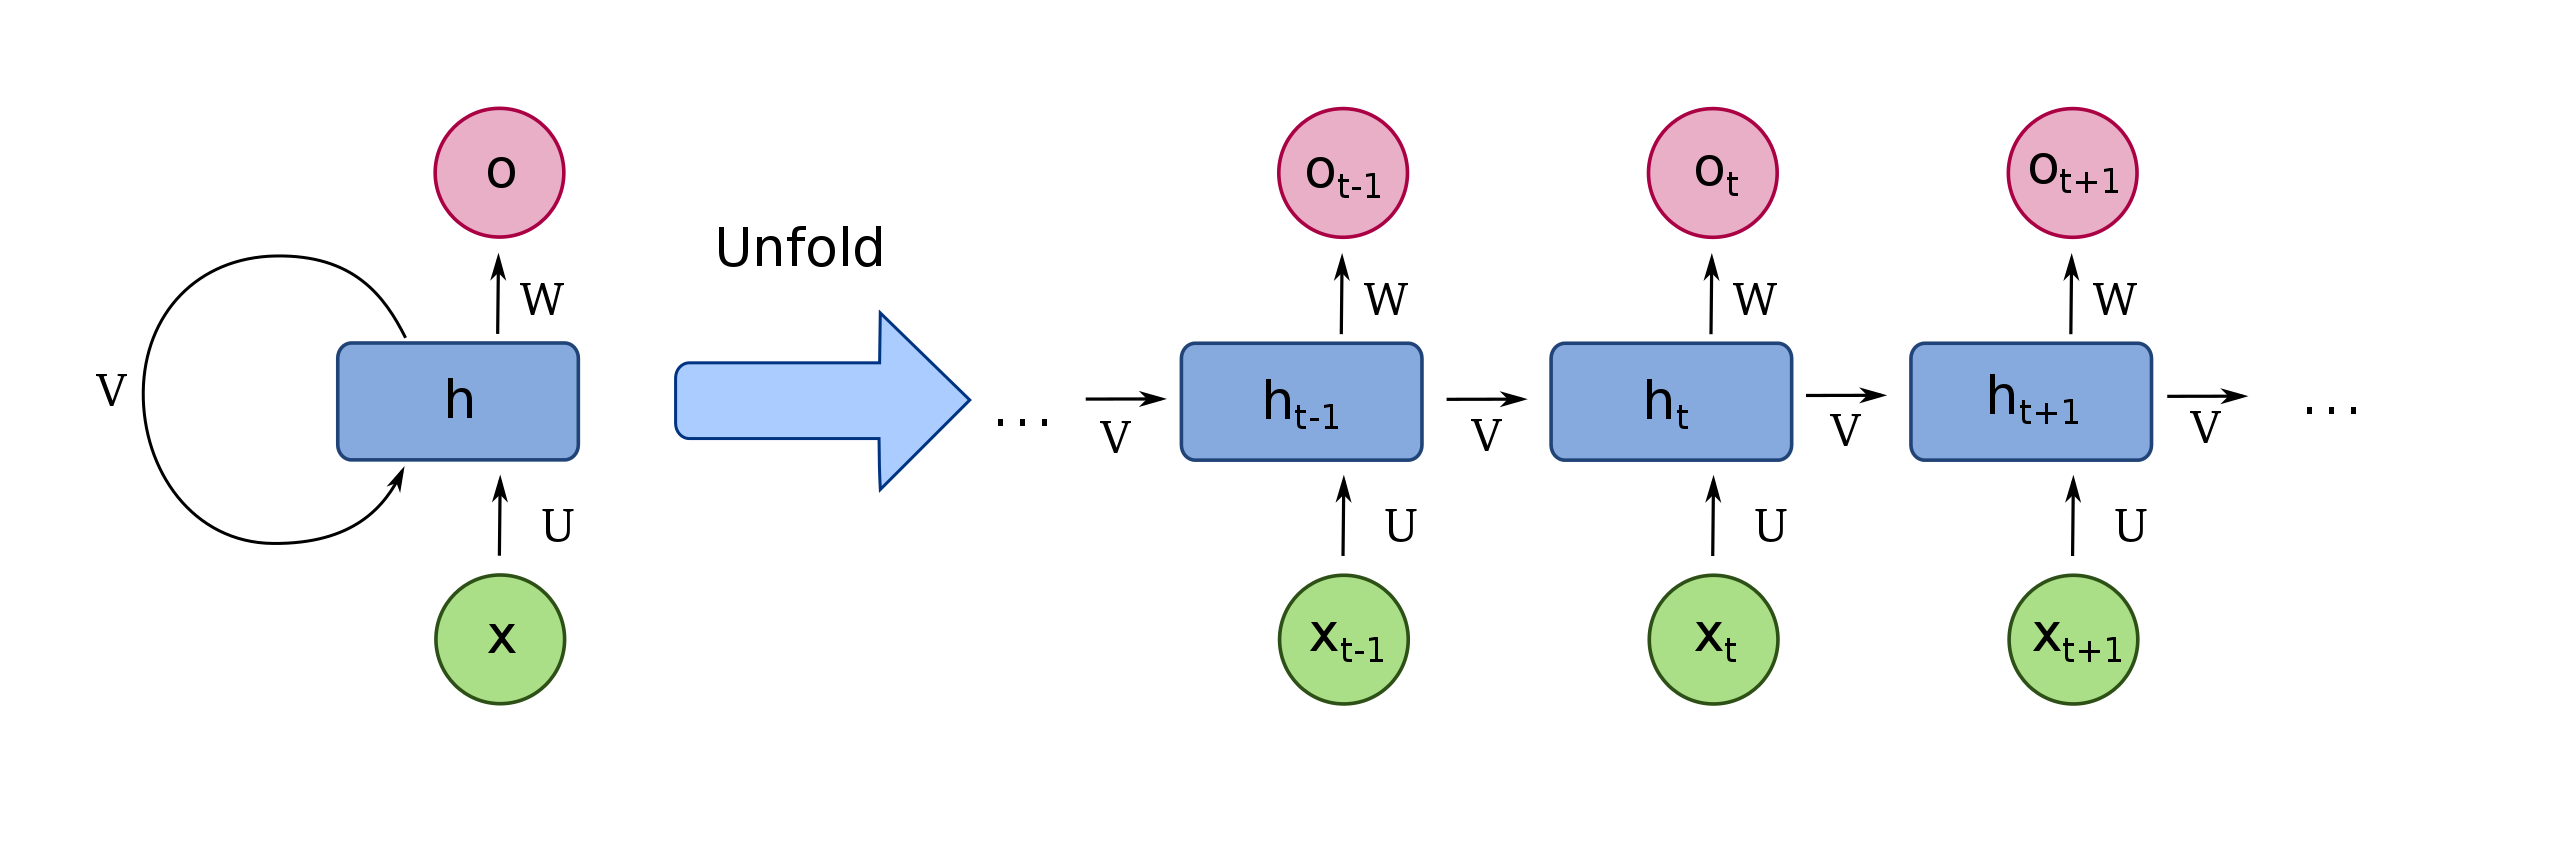
\includegraphics[width=1\linewidth]{img/rnn-unfold}
			\caption{Unfolded RNN structure \footnote{Source: \url{https://commons.wikimedia.org/wiki/File:Recurrent_neural_network_unfold.svg}}}
			\label{fig:rnn-unrolled}
		\end{figure}
	
		These simple/vanilla RNNs keep information from previous inputs by having an internal recurrent hidden state defined for each time step $t$ as:
		\begin{equation}
			h_t = g(Wx_t + Uh_{t-1} + b)
		\end{equation}
		where $x_t$ is the input vector for time $t$, $h_{t-1}$ is the hidden vector from the previous time step, $g$ is an appropriate activation function , and $W$, $U$, $b$  are learned parameters.s
		
		The vanilla RNNs however cannot keep the information for too long due to either exploding or vanishing gradients \cite{bengio1994learning}. Two models were proposed to minimize these effects -- LSTM \cite{hochreiter1997long} and GRU \cite{cho2014learning}, the latter being the main subject of this project.
	
	\section{Method} \label{sec:gru-intro}
		The GRU RNN is a slightly modified version of the LSTM RNN. It lowers the number of gates inside a single cell compared to LSTM because it lacks the forget gate. Even with smaller number of gates than LSTM, GRUs were proved to perform the same or even better on certain smaller datasets \cite{chung2014empirical}. Specifically it consists of 2 gates -- an update gate $z_t$ and a reset gate $r_t$. Each cell of this model still contains a hidden state defined by
		\begin{equation}\label{eq:gru-h_hat}
			\hat{h_t} = g(W_hx_t+U_h(r_t \odot h_{t-1}) + b_h)
		\end{equation}
		\begin{equation}\label{eq:gru-h}
			h_t = z_t \odot h_{t-1} + (1-z_t) \odot \hat{h_t}
		\end{equation}
		With the 2 gates being defined as
		\begin{equation}\label{eq:gru-z}
			z_t = \sigma (W_zx_t + U_zh_{t-1} + b_z)
		\end{equation}
		\begin{equation}\label{eq:gru-r}
			r_t = \sigma (W_rx_t + U_rh_{t-1} + b_r)
		\end{equation}
		The output of each cell is then defined as
		\begin{equation}
			\hat{y_t} = softmax(Vh_t + b_y)
		\end{equation}
	
		Where $\odot$ is Hadamard product and $\sigma$ is an element-wise \textit{sigmoid} function.
		
		The total loss for each time step $t$ can be calculated as
		\begin{equation}
			L_t = \sum -y_t \odot log(\hat{y_t})
		\end{equation}
	
		The overall loss is then sum of all partial losses $L = \sum_{t=1}^{s} L_t$, where $s$ is some sequence length.
		
		\subsection{Backpropagation} \label{sec:gru-backpropagation}
			To ensure learning of this model, the overall loss must be backpropagated over the whole network to update the weights accordingly. This is done using the Backpropagation through time (BPTT) algorithm \cite{mozer1995bptt}. BPTT computes the gradients in each timestamp backwards and sums them up. These gradients were computed using the following equations:
			\begin{equation}
				dy_t = \hat{y_t} - y_t
			\end{equation}
			\begin{equation}
				dV_t = dy_th_t^T
			\end{equation}
			\begin{equation}
				db_{y_t} = dy_t
			\end{equation}
			\begin{equation}
				dh_t = V^Tdy_t + dh_{t+1}
			\end{equation}
			\begin{equation}
				d\hat{h_t} = dh \odot (1-z_t)
			\end{equation}
			\begin{equation}
				d\hat{h_{l_t}} = d\hat{h_t} \odot tan'(\hat{h_t})
			\end{equation}
			
			Gradients for $W_h$, $U_h$, and $b_h$
			\begin{equation}
				dW_{h_t} = d\hat{h_{l_t}} x_t^T
			\end{equation}
			\begin{equation}
				dU_{h_t} = d\hat{h_{l_t}} (r_t \odot h_{t-1})^T
			\end{equation}
			\begin{equation}
				db_{h_t} = d\hat{h_{l_t}}
			\end{equation}
			
			\begin{equation}
				drhp_t = U_h^T d\hat{h_{l_t}}
			\end{equation}
			\begin{equation}
				dr_t = drhp_t \odot h_{t-1}
			\end{equation}
			\begin{equation}-rw-r--r-- sveatlo/sveatlo 23103 2022-01-02 12:47 docs/losses_dinos_adam_with_lr_h25_s25_e20_lr0005.png
				dr_{l_t} = dr * \sigma'(r_t)
			\end{equation}
		
			Gradients for $W_r$, $U_r$, and $b_r$
			\begin{equation}
				dW_{r_t} = dr_{l_t} x_t^T
			\end{equation}
			\begin{equation}
				dU_{r_t} = dr_{l_t} h_{t-1}^T
			\end{equation}
			\begin{equation}
				db_{r_t} = dr_{l_t}
			\end{equation}
			
			\begin{equation}
				dz_t = dh_t \odot (h_{t-1} - \hat{h_t})
			\end{equation}
			\begin{equation}
				dz_{l_t} = dz_t \sigma'(z_t)
			\end{equation}
		
			
			Gradients for $W_z$, $U_z$, and $b_z$
			\begin{equation}
				dW_{z_t} = dz_{l_t} x_t^T
			\end{equation}
			\begin{equation}
				dU_{z_t} = dz_{l_t} h_{t-1}^T
			\end{equation}
			\begin{equation}
				db_{z_t} = dz_{l_t}
			\end{equation}
		
			And for the next timestamp a new $dh_{t+1}$ is computed by summing up its partial gradients.
			\begin{equation}				
				dh_{t+1} = U_z dz_{l_t} + (dh_t \odot z_t) + (drhp_t \odot r_t) + U_r^T dr_{l_t}
			\end{equation}
				
		\subsection{Variants}
			Besides the basic GRU form as presented in \ref{sec:gru-intro}, there are 3 variants to the GRU networks \cite{dey2017gatevariants}:
			\begin{enumerate}
				\item \textbf{Type 1} uses only the previous hidden state and the bias
					\begin{equation}
						z_t = \sigma_g(U_{z} h_{t-1} + b_z)
					\end{equation}
					\begin{equation}
						r_t = \sigma_g(U_{r} h_{t-1} + b_r) 
					\end{equation}
				
				\item \textbf{Type 2} uses only the previous hidden state
					\begin{equation}
						z_t = \sigma_g(U_{z} h_{t-1})
					\end{equation}
					\begin{equation}
						r_t = \sigma_g(U_{r} h_{t-1}) 
					\end{equation}
				
				\item \textbf{Type 3} uses only the bias
					\begin{equation}
						z_t = \sigma_g(b_z)
					\end{equation}
					\begin{equation}
						r_t = \sigma_g(b_r) 
					\end{equation}
			\end{enumerate}
		
		%\subsection{Optimizer}
		%	As part of the implementation 2 optimizers were implemented -- Adagrad\cite{duchi2011adaptive} and Adam\cite{kingma2017adam}.
		%	
		%	\subsubsection{Adam}
		%   	\todo{}

	\section{Implementation} \label{sec:implementation}
		As stated in \ref{sec:introduction}, this project is mostly about getting deep knowledge of all internal operations during a training of a GRU network, therefore I decided against using any abstraction even for matrices operation as suggested after the project proposal. This means that the code cannot be run in HW accelerated environment such as using a GPU, but the practical usability is very limited either way, so this project doesn't suffer by this.
		
		The whole project is implemented completely in C++ without any external dependencies. The main function handles parameter parsing (see \ref{app:usage} for details), input file preprocessing and losses output (this is useful for plotting the loss progress).
		
		\paragraph{Performance} The fact that the model cannot be run on GPU is largely minimized thanks to compiler optimizations. Running the \texttt{g++} compiler with \texttt{-O3} flag turns on automatic vectorization, which greatly improves the operations on matrices. This is still slower than running on GPU/TPU but performs good enough for a project of this size.
		
		\paragraph{Preprocessing} The preprocessing includes loading the file data, splitting the data into chars, creating encoding for the characters (simple index-to-char encoding), and optionally converting the chars to lowercase, which can help with larger datasets (though it is limitted).
		
		\paragraph{Model} The main model is implemented in the \texttt{GRU} class which handles both forward and backward passes, sampling, paramters' values and updates as well as other minor responsibilities. Later a method for loading saved parameters could be added. The parameters are initialized using Xavier initialization, which should be favorable for non-linear activations \cite{kumar2017weight}.
		
		\paragraph{Matrix operations} For matrix operations I created a \texttt{Matrix} class which is templated so that either \texttt{double} or \texttt{float} data types can be used and handles all of the matrix operations needed in this project including addition, subtraction, matrix product, Hadamard product, etc.
		
	
	\section{Experimental Setup} \label{sec:setup}
		The experimental setup should contain all model and training hyperparameters, but also datasets and evaluation process descriptions (e.g. number of trained models per experiment or used metrics). 
		You could also include other implementation details such as used framework or computer parameters, where the models were trained and evaluated.
		
		\subsection{Datasets}
			Several different datasets were used for the traning, testing, and experiments. Here is a quick overview:
			\begin{itemize}
				\item \href{https://www.kaggle.com/kumazaki98/dinosaur-list}{Dinosaur names} - list of 1143 unique names of dinosaur names. Only list of names was supplied to the model for training
				\item Lorem ipsum - 40 paragraphs of generated Lorem ipsum text
				\item \href{https://www.kaggle.com/gulsahdemiryurek/harry-potter-dataset?select=Harry+Potter+1.csv}{Harry Potter 1 movie script} - subtitles from the 1st Harry Potter movie. Only the text was supplied to the model for training.
			\end{itemize}
		
		\subsection{Hyperparameters}
			The program allows for easy setting of hyperparameters:
			\begin{itemize}
				\item learning rate - regulates how much the gradients contribute to the weights/parameters
				\item sequence length - longer sequences allow for lengthier latent dependencies
				\item hidden size - can change the abstractness of the network and the amount of information that can be saved
			\end{itemize}
		
		\subsection{Optimizers}
			The project implements 2 different optimizers for updating the parameters' values -- AdaGrad \cite{duchi2011adaptive} Adam \cite{kingma2017adam}. I will not describe them here in detail, but the results can be seen in next section.
	
	\section{Results and Analysis} \label{sec:results}
		\subsection{Comparing optimizers}
			Comparing the Adam and AdaGrad optmizers, we can clearly see that the Adam optimizer converges faster, but the overall model performance doesn't change. Both tests were done on the dinosaur names dataset, with sequence length 25, hidden size 25, and learning rate of 0.1 in 10 training epochs.
			
			\begin{figure}[h]
				\centering
				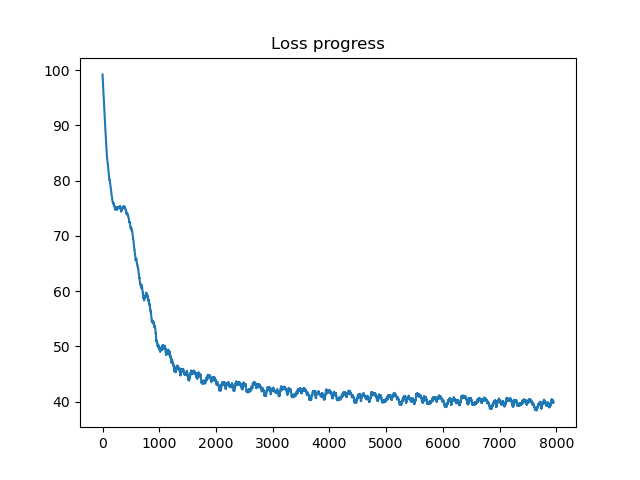
\includegraphics[width=\linewidth]{img/losses_dinos_adagrad_h25_s25_e10_lr01.png}
				\caption{Training with the AdaGrad optimizer (hidden size 25, sequence length 25, learning rate 0.1, 10 epochs)}
				\label{fig:lossesdinosadagradh25s25e10lr01}
			\end{figure}
		
			\begin{figure}[h]
				\centering
				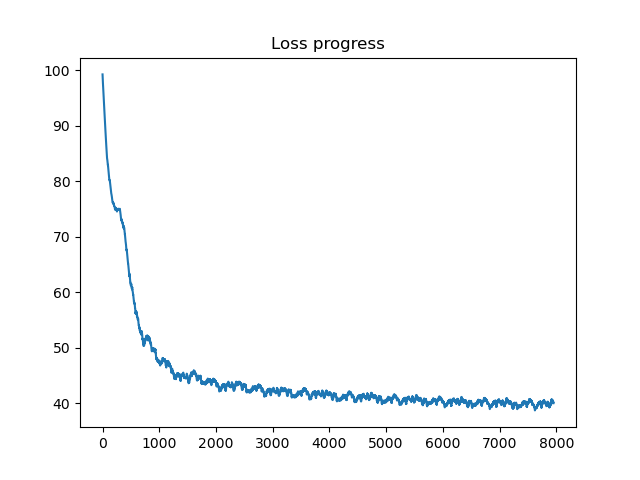
\includegraphics[width=\linewidth]{img/losses_dinos_adam_h25_s25_e10_lr01.png}
				\caption{Training with the Adam optimizer (hidden size 25, sequence length 25, learning rate 0.1, 10 epochs)}
				\label{fig:lossesdinosadamh25s25e10lr01}
			\end{figure}
		
		\subsection{Comparing results on different datasets}
			\paragraph{Dinosaur names} dataset has the best performance of all. This is probably thanks to it being relatively simple without complicated structure or names. In figure \ref{fig:dinos_output} we can see that the model successfully trained to capitalize the first letter on line and use suffixes such as \textit{-us} or \textit{-saurus}.
			
			\begin{figure}[h]
				\centering
				\textit{
					Tebcrekabevanius,
					Qarotischus,
					Sinocheus,
					Torpoophus,
					Uudesaurus,
					Tenstotolthus,
					Teoviceuuchus,
					Tanchiomisaurus,
					Therosaurus,
				}
				
				\caption{Generated dinosaur names (new lines replaced by commas)}
				\label{fig:dinos_output}
			\end{figure}
		
		
			\paragraph{Lorem ipsum} provides a challenge in the structure of the text -- it needs to be consistent with naturally varying length of the words and capital letters after full stops.  As we can see in fig. \ref{fig:lipsum_output}, the model can successfully generate a convincing pseudo-latin text.
			
			\begin{figure}[h]
				\centering
				
				\textit{
					Inque esse damiras egum, qua per soemquates et di it, quod ditera, comptane, de quo defere, quae risa dempota. Nam, cum res potest, iltio, ciobus inixi holast! Senem hobas, diri! qui esse. Damendo axcdit?
				}
				
				\caption{Generated lorem ipsum text}
				\label{fig:lipsum_output}
			\end{figure}
		
			\paragraph{Natural language} is the most challenging because it needs to keep both the structure of natural text, generate sensible words and keep context. As we can see in fig. \ref{fig:harry_output}, the model cannot handle this scenario. Even though it mostly correctly generates the words including common names and places, the text as a whole is nonsense.
			
			I believe this is mainly limitation of the model generating the text character by character, therefore having a shorter span of information, and the encoding, which doesn't give the model any information about the meaning of the words. This test was run with sequence lengths of 25, 100, 200 without any significant change in the output.
						
			\begin{figure}[h]
				\centering
				
				\textit{
					"They and Dudley would Harry more at as eyes put Hogwarts undisting up the welled could of a minior Gringotts out omath haten therl thaught last ever yep around to his nose Grinnowin. How, been an' hoila right of brickad himmansis reastay; you his bas. Hogrif.
				}
				
				\caption{Generated natural text}
				\label{fig:harry_output}
			\end{figure}
	
	\section{Conclusion}
		In this project I successfully created a fully working GRU model from scratch.
		
		It can learn simple patterns from input datasets and generate new text character-by-character. As shown in \ref{sec:results} it is not enough for comprehensible text, but suffices for simpler datasets. It can also be further improved by alternating it to use words as its tokens instead of characters and using better encoding for the tokens themselves (e.g. word embeddings).
	
% Entries for the entire Anthology, followed by custom entries
\bibliographystyle{acl_natbib}
\nocite{*}
\bibliography{references}
	
\newpage
\appendix

\section{Usage manual}\label{app:usage}
	\subsection{Compilation}
		The program can be compiled using the included Makefile by running \texttt{make} in the project's root directory.
		
	\subsection{Parameters}
		The compiled binary takes several command-line options to change the hyperparameters without recompilation:
		\begin{itemize}
			\item[-h] print help
			\item[-f] Path to the dataset file which should be plain text (default: None, required)
			\item[-l] Learning rate (default: 0.01)
			\item[-e] Number of epochs for training (default: 10)
			\item[-i] Hidden size (default: 25)
			\item[-s] Sequence length (default: 25)
			\item[-o] Path to losses output file (default: None - do not output weights)
		\end{itemize}
	
	\subsection{Losses plot}
		To plot the losses from a losses output file, you can use the included \texttt{plot\_loss.py} script. It takes the losses file as argument and displays and saves a plot of the loss progress.


\end{document}
